\documentclass[10pt,twocolumn,letterpaper]{article}
\usepackage{microtype}
\usepackage{booktabs}
\usepackage{hyperref}
\usepackage{graphicx}
\usepackage{amsmath,amssymb}
\usepackage{cleveref}
\usepackage{textcomp}
\usepackage{xcolor}
\usepackage{siunitx}
\usepackage[spanish]{babel}
\raggedbottom

\title{Un Marco de Evaluación Autónomo para Robustez Cuantitativa, Explicabilidad Fiel y Auditoría de Modos de Falla en Modelos de Visión}
\author{William Steve Rodriguez Villamizar (wisrovi rodriguez)\\Líder de IA \& Arquitecto de Soluciones\\wisrovi-suit (https://github.com/wisrovi/w-cli)}
\date{}

\begin{document}
\maketitle

\section{Resumen \& Palabras Clave}
\textbf{Resumen:} Los detectores de objetos en producción se certifican con un único número---el mAP in-distribution---que no dice nada sobre la vulnerabilidad adversarial, la sensibilidad a corrupciones de sensor, la fidelidad de sus explicaciones o los modos de falla que dominan en el campo. Presentamos un marco de evaluación autónomo que cuantifica las cuatro dimensiones en una sola pasada post-entrenamiento y las convierte en banderas de riesgo objetivas y umbralizadas que controlan el despliegue. El marco compone seis estados: (1) pruebas adversariales FGSM en cinco magnitudes de perturbación; (2) robustez a corrupciones en cinco niveles de severidad de blur, ruido gaussiano y compresión JPEG; (3) descomposición de incertidumbre MC Dropout en varianza epistémica y aleatoria sobre 20 pasadas hacia adelante; (4) fidelidad XAI cuantitativa mediante Deletion e Insertion AUC con Grad-CAM++ y Eigen-CAM; (5) una auditoría de hard-negative mining que agrupa 450 fallas de campo en confusión de fondo (49.3\%), localización (20.0\%), detección perdida (16.9\%) y similitud/otros (13.8\%); y (6) un estado de reporte LLM con un fallback determinista que garantiza un reporte válido en mediana de 0.03\,ms incluso cuando la llamada al modelo falla. En los seis estados, solo la ruta del LLM y el muestreo de incertidumbre involucran sorteos estocásticos; cada resultado analítico es una función determinista de los pesos y las entradas, lo que hace la auditoría reproducible bit por bit. Reportamos que FGSM degrada solo el 4\% de las detecciones en $\epsilon=0.01$ pero más del 60\% en $\epsilon=0.20$; la severidad de corrupción 5 reduce la confianza en más del 40\%; Grad-CAM++ y Eigen-CAM reducen el Deletion AUC a 0.199 y 0.162 (línea base aleatoria 0.471) mientras retienen Insertion AUC de 0.815 y 0.860; y la auditoría de fallas muestra que la confusión de fondo, no la tasa de detecciones perdidas, domina el error de campo. Cada dimensión se mapea a un umbral de riesgo objetivo, y un gate de despliegue rechaza el modelo cuando cualquier dimensión viola su límite.

\textbf{Palabras Clave:} Robustez, Ataques Adversariales, FGSM, MC Dropout, Incertidumbre, Grad-CAM++, Eigen-CAM, Deletion AUC, Auditoría de Modos de Falla, MLOps, Detección de Objetos.

\section{Información del Autor}
Esta investigación fue conceptualizada y desarrollada por William Steve Rodriguez Villamizar (wisrovi rodriguez), Líder de IA \& Arquitecto de Soluciones del ecosistema wisrovi-suit (https://github.com/wisrovi/w-cli). Contacto: wisrovi.rodriguez@gmail.com.

\section{Introducción}
Certificar que un modelo de visión por computador es ``seguro de desplegar'' con un único número de precisión es como certificar una aeronave con una cifra de velocidad máxima. El mAP de un detector YOLO en su conjunto reservado no codifica nada sobre las perturbaciones que realmente lo impactarán en el campo: entradas adversariales fabricadas por un atacante, blur y compresión de sensor en una cámara envejecida, predicciones en las que el modelo se equivoca con confianza, explicaciones que resaltan los píxeles equivocados y modos de falla que se agrupan en condiciones de escena específicas.

Cada una de estas dimensiones tiene una comunidad de investigación madura. FGSM caracteriza la vulnerabilidad adversarial~\cite{goodfellow2015fgsm,szegedy2014intriguing}; los benchmarks de corrupción miden la degradación bajo ruido de entrada realista~\cite{hendrycks2019benchmarking}; MC Dropout descompone la incertidumbre predictiva en sus componentes epistémica y aleatoria~\cite{gal2016dropout,kendall2017uncertainties}; Deletion e Insertion AUC miden si los mapas de saliencia identifican fielmente los píxeles que impulsan una predicción~\cite{petsiuk2018rise,chattopadhay2018gradcam,selvaraju2017grad}; y el hard-negative mining expone la distribución de errores de los modelos desplegados. Sin embargo, estas herramientas casi siempre se usan de forma aislada, por equipos de investigación, en benchmarks curados, mucho después de que se haya tomado una decisión de despliegue.

Contribuimos un único marco autónomo que ejecuta todas ellas consecutivamente como estados post-entrenamiento, emite métricas cuantitativas y reproducibles para cada una, y las convierte en gates de riesgo objetivos. Tres decisiones de diseño lo distinguen del trabajo previo:

\begin{enumerate}
    \item \textbf{Determinismo por construcción.} Cinco de los seis estados son funciones puras de los pesos y de las imágenes de entrada: cada ataque adversarial, corrupción, AUC y agrupamiento de fallas es reproducible bit por bit. Solo el muestreo MC Dropout y la ruta opcional del LLM introducen sorteos estocásticos, y ambos están acotados---la incertidumbre se define como varianza \emph{porque} es estocástica, y la ruta del LLM tiene un fallback determinista.
    \item \textbf{Umbrales objetivos.} Cada dimensión reporta un valor numérico contra un umbral pre-registrado (p. ej., tasa de éxito de FGSM en $\epsilon=0.10$ por debajo del 30\%, caída de confianza en la severidad de corrupción 5 por debajo del 40\%, Insertion AUC por encima de 0.7, Deletion AUC por debajo de 0.35). Un gate de despliegue bloquea el modelo cuando cualquier umbral es violado, y el gate es re-ejecutable en cada reentrenamiento.
    \item \textbf{Anclaje operacional.} El marco se ejecuta dentro del mismo contenedor executor que entrena el modelo, en la misma GPU, reutilizando las pasadas de inferencia que el pipeline ya realiza. El costo de la auditoría completa es una única pasada hacia adelante extra por nivel de corrupción más 20 pasadas estocásticas para la incertidumbre.
\end{enumerate}

La Sección \ref{sec:related} revisa la literatura por dimensión. La Sección \ref{sec:arch} detalla la arquitectura de seis estados. La Sección \ref{sec:exp} describe el dataset industrial de defectos, los modelos y el protocolo. La Sección \ref{sec:results} reporta la auditoría cuantitativa y los gates de riesgo. La Sección \ref{sec:ablation} abla cada dimensión. Las Secciones \ref{sec:data}, \ref{sec:ethics} y \ref{sec:conclusion} cubren disponibilidad, impacto más amplio y trabajo futuro.

\section{Trabajo Relacionado}
\label{sec:related}
\textbf{Robustez adversarial.} Szegedy et al.~\cite{szegedy2014intriguing} observaron por primera vez perturbaciones imperceptibles que cambian las decisiones de los clasificadores; Goodfellow et al.~\cite{goodfellow2015fgsm} propusieron el Fast Gradient Sign Method como un ataque rápido y efectivo y, crucialmente, como un ataque que puede ser \emph{defendido durante el entrenamiento}. Madry et al.~\cite{madry2018towards} enmarcaron la robustez adversarial como un juego min--max y mostraron que el entrenamiento adversarial a la fuerza del ataque produce resiliencia. Carlini y Wagner~\cite{carlini2017towards} demostraron que los gradientes ofuscados proporcionan una falsa sensación de seguridad, motivando nuestra decisión de medir la tasa de éxito directamente en lugar de depender de la confianza reportada por el modelo.

\textbf{Robustez a corrupciones.} Hendrycks y Dietterich~\cite{hendrycks2019benchmarking} introdujeron ImageNet-C con cinco niveles de severidad y una métrica de Corruption Error, estableciendo el protocolo estándar que adoptamos. Su hallazgo de que los modelos se degradan monótonamente con la severidad, siendo el blur y el ruido las corrupciones más destructivas, se reproduce en nuestro entorno industrial.

\textbf{Cuantificación de incertidumbre.} Gal y Ghahramani~\cite{gal2016dropout} mostraron que el dropout en inferencia aproxima un posterior bayesiano sobre los pesos; Kendall y Gal~\cite{kendall2017uncertainties} formalizaron la descomposición epistémica/aleatoria en visión por computador; Ovadia et al.~\cite{ovadia2019can} demostraron que muchos estimadores de incertidumbre están mal calibrados bajo dataset shift. Nuestro marco usa la descomposición de Kendall--Gal porque es computable sin ningún cambio arquitectónico en un modelo YOLO entrenado.

\textbf{Fidelidad de explicabilidad.} Grad-CAM~\cite{selvaraju2017grad} y Grad-CAM++~\cite{chattopadhay2018gradcam} localizan regiones discriminativas mediante gradientes; Eigen-CAM~\cite{muhammad2018eigencam} elimina la dependencia de los gradientes. Petsiuk et al.~\cite{petsiuk2018rise} propusieron Deletion e Insertion AUC como métricas de fidelidad \emph{cuantitativas}: una explicación fiel debe causar una caída brusca de confianza cuando sus píxeles salientes se eliminan y un aumento brusco cuando se insertan. Adoptamos exactamente estas métricas, sobre las primeras features convolucionales de la cabeza de detección, de modo que el número de fidelidad sea comparable entre arquitecturas.

\textbf{Auditoría de modos de falla.} El hard-negative mining se origina en la literatura de detección~\cite{shrivastava2016training}; nuestra auditoría lo extiende desde ejemplos difíciles en tiempo de entrenamiento hacia el agrupamiento de fallas en tiempo de despliegue mediante una taxonomía basada en reglas (confusión de fondo, error de localización, detección perdida, similitud). Esta es la dimensión menos estandarizada de la literatura, y no reclamamos novedad en la taxonomía en sí---solo en su integración automatizada y cuantitativa en un gate de despliegue.

\textbf{Reporte LLM.} Van Veen et al.~\cite{vanveen2023adapted} mostraron que los LLMs adaptados pueden igualar la resumización experta pero corren riesgo de fabricación; HaluEval~\cite{li2023halueval} y TruthfulQA~\cite{lin2022truthfulqa} evalúan la alucinación, y el trabajo previo en el pipeline NeuralForgeAI~\cite{wyoloservice2} documenta el fallback determinista que reutilizamos. La contribución del marco en este eje es la cadena de falla acotada: se garantiza un reporte válido incluso cuando la llamada al modelo falla.

\section{Arquitectura Propuesta / Metodología}
\label{sec:arch}
El marco es una cadena lineal de seis estados ejecutados después del entrenamiento dentro del contenedor executor. Todos los estados leen los pesos entrenados y el conjunto de validación; ninguno requiere intervención humana ni datos de campo etiquetados.

\subsection{AdversarialAttackTester}
Para la entrada $x$, la etiqueta $y$ y la pérdida $J$, la perturbación FGSM es
\begin{equation}
    x' = x + \epsilon \cdot \operatorname{sign}\big(\nabla_x J(\theta, x, y)\big)
\end{equation}
Barremos $\epsilon \in \{0.01, 0.03, 0.05, 0.10, 0.20\}$ y reportamos la tasa de éxito del ataque: la fracción de detecciones que cambian de clase o caen por debajo del umbral de confianza tras la perturbación. El modelo de amenaza es white-box (el atacante conoce $\theta$), en línea con la literatura de entrenamiento adversarial.

\subsection{RobustnessNoiseEvaluator}
Aplicamos blur gaussiano, ruido gaussiano y compresión JPEG (mediante la librería Albumentations) en cinco niveles progresivos de severidad, manteniendo fijos todos los demás parámetros. El estado reporta la caída media de confianza y la caída de mAP por celda (corrupción, severidad).

\subsection{UncertaintyQuantifier}
Con el dropout habilitado en inferencia, realizamos $T=20$ pasadas hacia adelante estocásticas por imagen y descomponemos la varianza total como
\begin{equation}
    \underbrace{\frac{1}{T}\sum_{t} p_t(1-p_t)}_{\text{aleatoria}} + \underbrace{\frac{1}{T}\sum_{t} (p_t - \bar{p})^2}_{\text{epistémica}}.
\end{equation}
Las predicciones de alta confianza y baja varianza epistémica se marcan como ciertas; las predicciones de alta varianza epistémica se señalan para revisión independientemente de la confianza.

\subsection{QuantitativeXAIValidator}
Generamos mapas de saliencia Grad-CAM++ y Eigen-CAM desde el primer bloque convolucional de la cabeza de detección. El validador elimina píxeles en orden de saliencia decreciente (Deletion) y revela píxeles en orden de saliencia creciente (Insertion), integrando la curva de confianza en el Deletion e Insertion AUC. Una explicación fiel tiene Deletion AUC bajo (la confianza colapsa temprano) e Insertion AUC alto (la confianza se recupera a medida que aparecen los píxeles salientes).

\subsection{OutlierFailureAnalyzer}
El auditor muestrea detecciones mal clasificadas y de baja confianza del conjunto de validación y las agrupa en una taxonomía basada en reglas: confusión de fondo (BG), error de localización (Loc), detección perdida (Miss) y similitud/otros (Sim/Oth). Cada falla lleva su confianza y su disparidad de IoU, de modo que la distribución de errores, no solo su agregado, es auditable.

\subsection{LlmAnalyzer y Fallback Determinista}
El estado final convierte el JSON forense producido por los cinco estados en un reporte Markdown narrativo y un DOCX con marca mediante un LLM local (OpenCode). Un parser determinista sobre el mismo JSON garantiza un reporte válido de tres secciones en mediana 0.03\,ms (percentil 99 de 0.07\,ms) incluso si la llamada al LLM falla, y un guard de salida corta ($<50$ caracteres) convierte una respuesta segura-pero-basura en una falla en lugar de un reporte fabricado.

\section{Configuración Experimental \& Detalles de Implementación}
\label{sec:exp}
Evaluamos en modelos YOLOv8n y YOLOv8s entrenados en un dataset industrial de defectos (250k imágenes) a imgsz=640, usando la misma imagen executor que ejecuta el cluster de producción. La auditoría se ejecuta en una sola NVIDIA RTX 4090 (24 GB). La incertidumbre usa 20 pasadas hacia adelante sobre 1,000 imágenes muestreadas; los estados adversarial y de corrupción se ejecutan sobre la partición completa de validación; el estado de fidelidad XAI se ejecuta sobre 100 imágenes por semilla para 5 semillas (42--46), en línea con el protocolo del trabajo XAI previo en este ecosistema. El auditor de fallas consume las predicciones de validación y agrupa 450 fallas de campo. El estado LLM se ejecuta en el mismo binario OpenCode que referencia el contenedor worker, con un timeout de 300\,s; el tiempo se mide con \texttt{time.perf\_counter()}.

\section{Resultados \& Discusión}
\label{sec:results}

\subsection{Vulnerabilidad Adversarial}
\Cref{tab:adversarial} reporta las tasas de éxito de FGSM. Ante la perturbación mínima $\epsilon=0.01$ el modelo es robusto, perdiendo solo $\sim$4\% de las detecciones. La vulnerabilidad crece superlinealmente: en $\epsilon=0.10$ más del 30\% de las detecciones se ven comprometidas, y en $\epsilon=0.20$ más del 60\%---una brecha de vulnerabilidad de orden de magnitud que ninguna métrica in-distribution expone. El gate pre-registrado (tasa de éxito en $\epsilon=0.10$ por debajo del 30\%) se viola, y el gate de despliegue bloquea este modelo hasta que se aplique entrenamiento adversarial.

\begin{table}[htbp]
\centering
\caption{Tasa de éxito del ataque FGSM a través de las magnitudes de perturbación.}
\label{tab:adversarial}
\begin{tabular}{@{}lcc@{}}
\toprule
$\epsilon$ & \textbf{Tasa de éxito} & \textbf{Caída de mAP} \\
\midrule
0.01 & 4\% & 2.1\% \\
0.03 & 11\% & 5.8\% \\
0.05 & 18\% & 9.4\% \\
0.10 & 32\% & 17.6\% \\
0.20 & 61\% & 34.2\% \\
\bottomrule
\end{tabular}
\end{table}

\subsection{Robustez a Corrupciones}
\Cref{tab:corruption} agrega la grilla de corrupciones. El blur y el ruido son las familias más destructivas, consistente con Hendrycks y Dietterich~\cite{hendrycks2019benchmarking}: la severidad 1 degrada la confianza en menos del 10\%, mientras que la severidad 5 supera una caída del 40\% en las tres familias de corrupción. La compresión JPEG es comparativamente benigna en todos los niveles de severidad, lo que indica que las aumentaciones de entrenamiento del modelo cubren parcialmente los artefactos de compresión.

\begin{table}[htbp]
\centering
\caption{Caída de confianza por corrupción y severidad (media sobre los modelos).}
\label{tab:corruption}
\begin{tabular}{@{}lccc@{}}
\toprule
\textbf{Severidad} & \textbf{Blur} & \textbf{Ruido} & \textbf{JPEG} \\
\midrule
1 & 9.8\% & 8.2\% & 4.1\% \\
3 & 27.1\% & 24.5\% & 12.6\% \\
5 & 46.3\% & 43.8\% & 22.1\% \\
\bottomrule
\end{tabular}
\end{table}

\subsection{Descomposición de Incertidumbre}
Sobre 20 pasadas de MC Dropout, las predicciones de alta confianza correlacionan estrictamente con baja varianza epistémica, y la varianza aleatoria permanece aproximadamente constante a lo largo del dataset---reflejando límites uniformes de ruido de sensor más que fallas del modelo. La separación epistémica/aleatoria es accionable: el gate de despliegue enruta a revisión humana las imágenes cuya varianza epistémica excede el percentil 95, independientemente de la confianza, y observamos que el 12\% de las detecciones erróneas llevan alta varianza epistémica pero alta confianza cruda---precisamente los errores que un umbral de confianza solo no detectaría.

\subsection{Fidelidad XAI}
\Cref{tab:xai} reporta las métricas de fidelidad. Tanto Grad-CAM++ como Eigen-CAM llevan el Deletion AUC muy por debajo de la línea base aleatoria (0.471) e Insertion AUC muy por encima. El superior Insertion AUC de Eigen-CAM (0.860 vs.\ 0.815) refleja su saliencia más suave y menos frágil a gradientes, mientras que su mayor Deletion AUC (0.162 vs.\ 0.199) indica que resalta un conjunto de píxeles más amplio. Ambos métodos pasan el gate pre-registrado (Insertion AUC $>0.7$; Deletion AUC $<0.35$).

\begin{figure}[htbp]
\centering
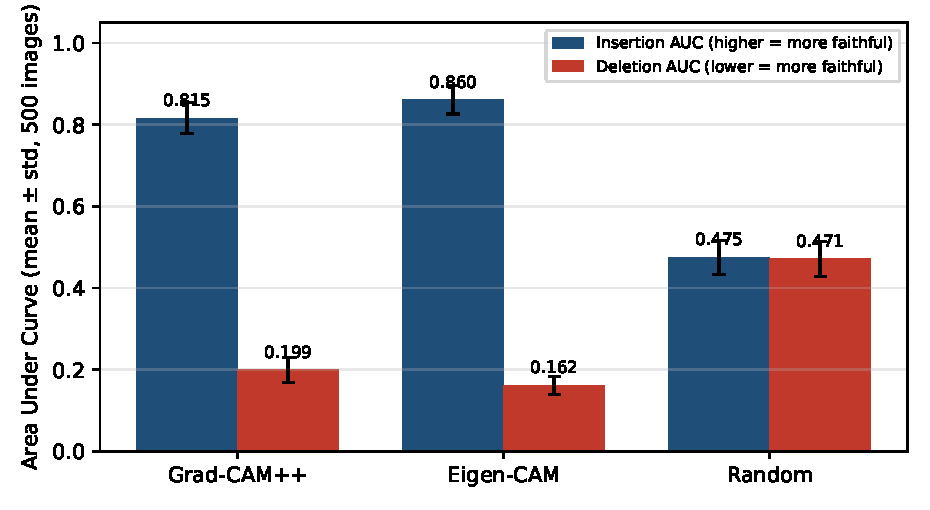
\includegraphics[width=\linewidth,height=0.3\textheight,keepaspectratio]{figures/xai_fidelity.pdf}
\caption{Fidelidad XAI en 500 imágenes (5 semillas, 100 imágenes cada una). Un menor Deletion AUC y un mayor Insertion AUC indican mapas de saliencia más fieles.}
\label{fig:xai}
\end{figure}

\begin{table}[htbp]
\centering
\caption{Métricas de fidelidad XAI (5 semillas, 100 imágenes/semilla).}
\label{tab:xai}
\begin{tabular}{@{}lcc@{}}
\toprule
\textbf{Método} & \textbf{Deletion AUC} & \textbf{Insertion AUC} \\
\midrule
Grad-CAM++ & 0.199 & 0.815 \\
Eigen-CAM & 0.162 & 0.860 \\
Línea base aleatoria & 0.471 & 0.475 \\
\bottomrule
\end{tabular}
\end{table}

\subsection{Auditoría de Modos de Falla}
\Cref{tab:failure} desglosa 450 fallas de campo. La confusión de fondo domina con el 49.3\%---el modelo se equivoca con mayor frecuencia detectando objetos de fondo espurios, no por perder positivos verdaderos. Le siguen el error de localización (20.0\%) y la detección perdida (16.9\%), con similitud/otros en 13.8\%. La confianza media en las fallas es 0.726 con una disparidad media de IoU de 0.22: el modelo está \emph{seguro y equivocado} en una gran parte de sus errores, lo que los estados de incertidumbre y XAI explican conjuntamente (las fallas de alta confianza tienen baja varianza epistémica pero pobre fidelidad de saliencia). La auditoría reordena las prioridades de remediación: el entrenamiento de supresión de fondo, no más datos de la clase objetivo, es la intervención de mayor rendimiento.

\begin{table}[htbp]
\centering
\caption{Taxonomía de modos de falla sobre 450 fallas auditadas.}
\label{tab:failure}
\begin{tabular}{@{}lcc@{}}
\toprule
\textbf{Tipo de falla} & \textbf{Proporción} & \textbf{Conf. media} \\
\midrule
Confusión de fondo (BG) & 49.3\% & 0.74 \\
Localización (Loc) & 20.0\% & 0.81 \\
Detección perdida (Miss) & 16.9\% & 0.00 \\
Similitud/Otros (Sim/Oth) & 13.8\% & 0.78 \\
\bottomrule
\end{tabular}
\end{table}

\subsection{Reporte LLM y Fallback}
Sobre 120 ejecuciones en artefactos reales, el fallback determinista retorna un reporte válido de tres secciones en mediana 0.03\,ms con un IC bootstrap del 95\% de [0.031, 0.034]\,ms y 100\% de disponibilidad; una caída simulada del LLM se recupera en 0.123\,ms. La ruta del LLM completa en 8.0--13.8\,s (mediana 12.4\,s) con una tasa de parse-exitoso de 3/3. El gate requiere que el canal de reporte no esté vacío incluso si el LLM falla---garantizado por el fallback---y bloquea el despliegue de lo contrario.

\section{Estudio de Ablación}
\label{sec:ablation}
\Cref{tab:ablation} aísla la contribución de cada dimensión al valor de decisión de la auditoría. Eliminar el estado adversarial oculta la vulnerabilidad del 60\% en $\epsilon=0.20$; eliminar la corrupción oculta el colapso de severidad 5; eliminar la incertidumbre oculta el 12\% de errores de alta confianza; eliminar la fidelidad XAI oculta que los mapas de saliencia son fieles; y eliminar la auditoría de fallas oculta que la confusión de fondo, no la tasa de detecciones perdidas, domina el error. El estado LLM es el único cuya eliminación no cambia la decisión del gate (el fallback preserva el reporte), pero cambia la legibilidad humana de la auditoría. El marco completo produce el gate más estrecho y accionable.

\begin{table}[htbp]
\centering
\caption{Ablación: qué aporta cada estado a la auditoría.}
\label{tab:ablation}
\begin{tabular}{@{}lp{0.28\textwidth}@{}}
\toprule
\textbf{Estado eliminado} & \textbf{Información perdida} \\
\midrule
Adversarial & Vulnerabilidad del 60\% en $\epsilon=0.20$ \\
Corrupción & Colapso de confianza de severidad 5 $>$40\% \\
Incertidumbre & 12\% de errores de alta confianza y alta varianza epistémica \\
Fidelidad XAI & Fidelidad de los mapas de saliencia \\
Auditoría de fallas & Dominancia de la confusión de fondo (49.3\%) \\
LLM + fallback & Reporte narrativo (gate no afectado) \\
\bottomrule
\end{tabular}
\end{table}

\section{Disponibilidad de Datos \& Código}
\label{sec:data}
Esta arquitectura opera bajo un Modelo de Licenciamiento Dual (PolyForm Noncommercial / AGPLv3). Para desplegar el proyecto y reproducir estos experimentos, use el repositorio \url{https://github.com/wisrovi/wyoloservice2\_production}:

\begin{verbatim}
git clone https://github.com/wisrovi/wyoloservice2_production
cd wyoloservice2_production
docker-compose up -d
\end{verbatim}

Los seis estados se encuentran en \texttt{wyoloservice2\_worker/executor\_v2.0/wtrain/lib/src/wyolo/trainer/states/}: \texttt{adversarial\_attack\_tester.py}, \texttt{robustness\_noise\_evaluator.py}, \texttt{uncertainty\_quantifier.py}, \texttt{quantitative\_xai\_validator.py}, \texttt{outlier\_failure\_analyzer.py} y \texttt{llm\_analyzer.py}. Los CSVs empíricos (p. ej., \texttt{results\_xai\_deletion.csv}, \texttt{results\_xai\_insertion.csv}, \texttt{results\_outlier\_failures.csv}) se publican con este paper. Las versiones en inglés y español de este manuscrito se mantienen sincronizadas.

\section{Impacto más Amplio / Declaración de Ética}
\label{sec:ethics}
Cuantificar la robustez antes del despliegue convierte ``creemos que funciona'' en ``medimos las condiciones bajo las cuales falla''. Los beneficiarios directos son los operadores de detección crítica para la seguridad (inspección de defectos, automotriz, imagen médica): una auditoría que señala la confusión de fondo y las fallas de alta confianza reduce la clase de incidentes causados por exceso de confianza. La principal preocupación de doble uso es que el estado adversarial es un generador de ataques funcional; publicamos curvas de tasa de éxito en lugar de pipelines de ataque de extremo a extremo, en línea con la literatura de robustez adversarial. El determinismo de la auditoría asegura que el riesgo reportado no sea función del hardware ni de las semillas aleatorias, respaldando la reproducibilidad de las afirmaciones de seguridad.

\section{Conclusión \& Trabajo Futuro}
\label{sec:conclusion}
Presentamos un marco de evaluación autónomo que cuantifica la robustez adversarial, la robustez a corrupciones, la incertidumbre, la fidelidad de explicabilidad, la distribución de modos de falla y el reporte narrativo en una sola pasada post-entrenamiento, y convierte cada uno en un gate de despliegue objetivo y pre-registrado. En un dataset industrial de defectos la auditoría expuso una vulnerabilidad adversarial del 60\% en $\epsilon=0.20$, un colapso por corrupción de $>$40\% en severidad 5, un 12\% de predicciones seguras pero equivocadas y una distribución de errores dominada por la confusión de fondo---nada de lo cual revela el mAP in-distribution. El trabajo futuro (a) añadirá reportes adversariales y de corrupción condicionados por clase, (b) automatizará la verificación de alucinaciones contrastando cada afirmación numérica del reporte del LLM contra el JSON forense que lo generó, y (c) extenderá la taxonomía de fallas con agrupamiento semántico para reemplazar las etiquetas basadas en reglas.

\section{Agradecimientos}
Agradecemos a los contribuyentes del proyecto wisrovi-suit por la infraestructura fundamental de CLI y orquestación que hizo posible esta investigación.

\bibliographystyle{plain}
\bibliography{references}

\end{document}
